% !TEX root=/home/tavant/these/manuscript/src/manuscript.tex

% \FloatBarrier

\section{Comparison of the sheath model with PIC simulations} \label{subsec-picandmodel}

  % \begin{figure}[hbt]
  %   \centering
  %   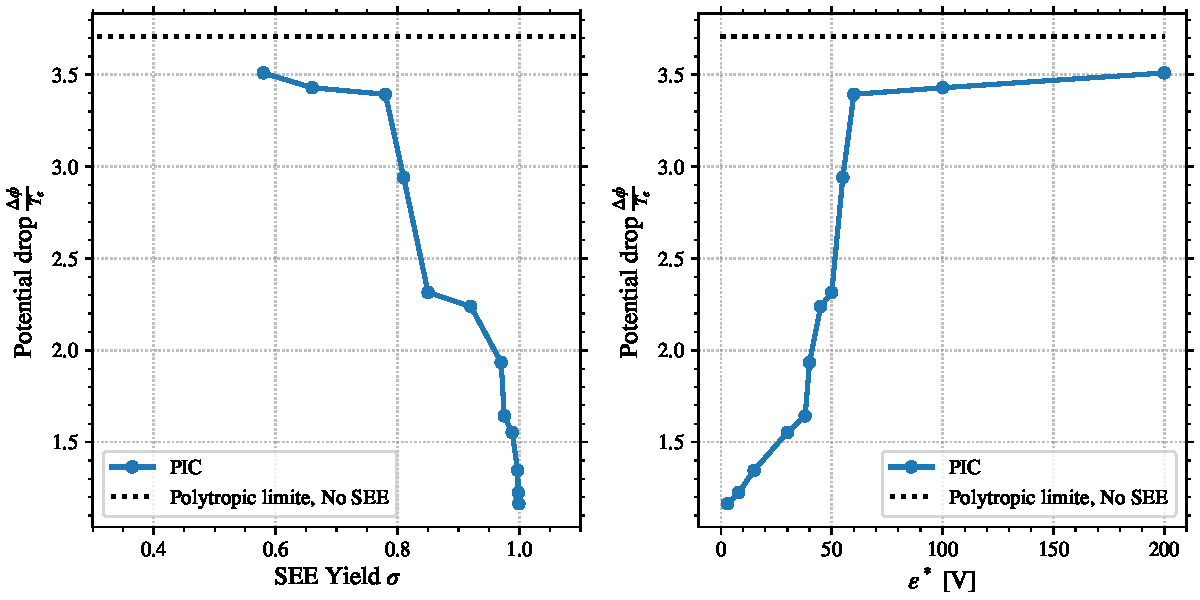
\includegraphics[width=\textwidth]{dphi_polytropic_noSEE}
  %   \caption{PIC simulation results (with SEE) compared to the polytropic limit without SEE.}
  %   \label{fig-polytropic_pic_noSEE}
  % \end{figure}
  % 
  % \begin{figure}[hbt]
  %   \centering
  %   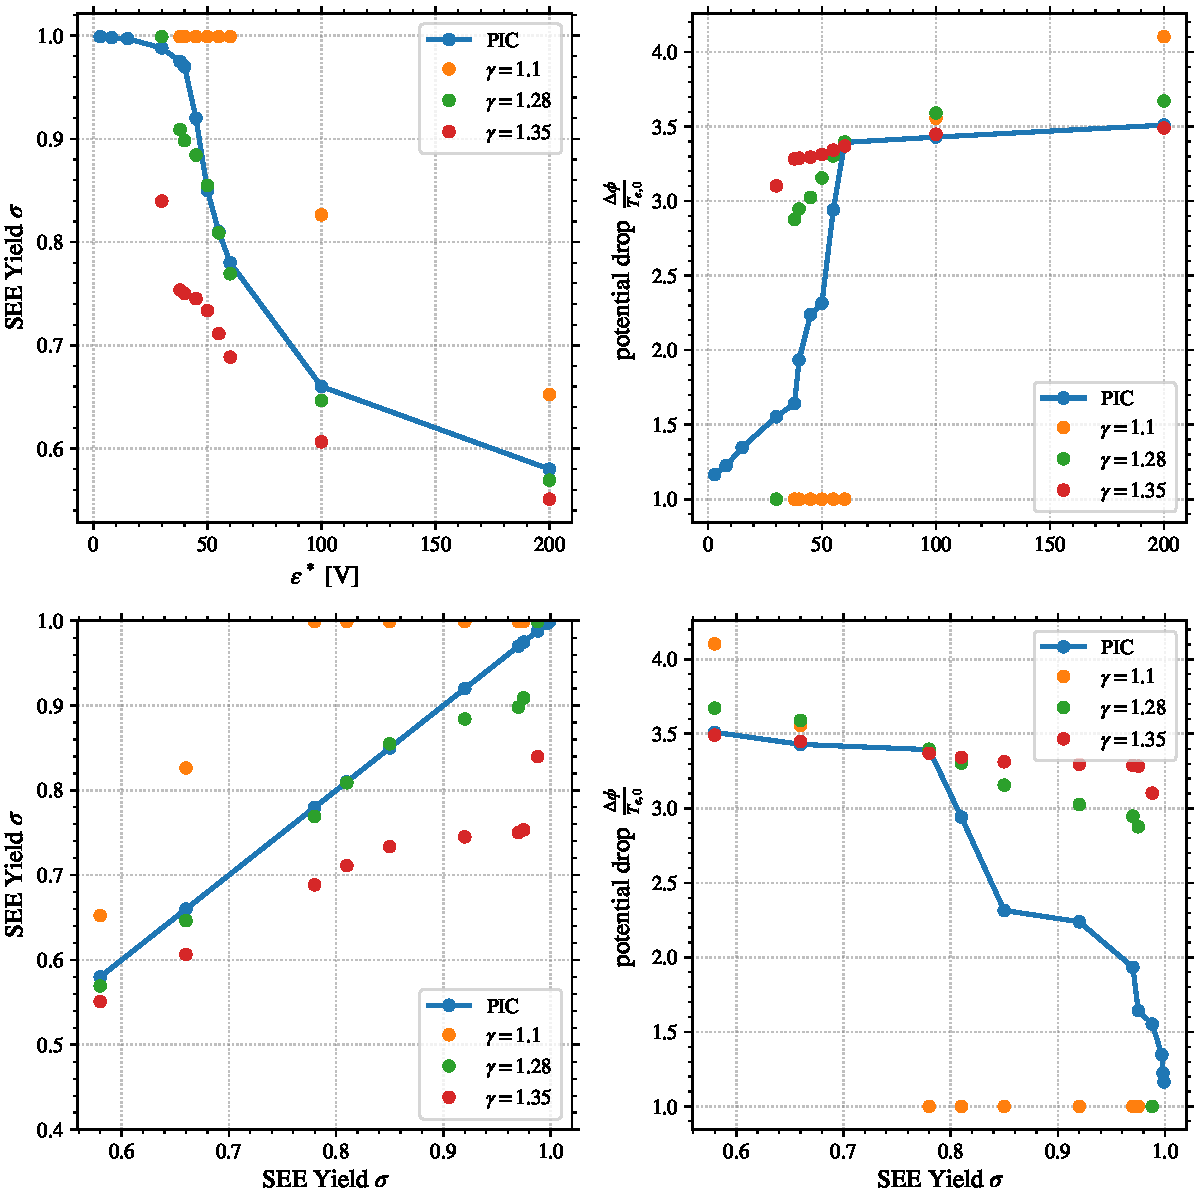
\includegraphics[width=\textwidth]{Summary_polytropic_SEE.pdf}
  %   \caption{Comparison of the PIC simulation results with the polytropic model with SEE.}
  %   \label{fig-polytropic_see_summary}
  % \end{figure}

  We compare in this section the characteristics of the plasma wall interaction observed in the \ac{PIC} simulations with the fluid model developed in \cref{sec-fluid_poly_see}.
  We first compare the mean values in the parametric study over the crossover energy $\crover$, then we investigate the oscillations of regime {\bf II}.

  \subsection{Parametric study of the modified sheath model} \label{subsec-param_sheath_see}

    The variables of interest to characterize the plasma-wall interaction are the averaged electron emission rate $\rate$ and the plasma potential drop to the wall.
    The only inputs of the modified sheath model are the electron mean temperature in the bulk $\Teb$, as well as the polytropic index $\gamma$.
    As seen in \cref{subsec-fluid_see_polyfit}, the polytropic index of the electron population is measured in the \ac{PIC} simulations to be $\gamma=1.35$.
    However, the electrons going toward the wall present a different index, measured from the bulk \ac{EVDF} to $\gamma=1.28$.
    These two values will be compared.

    Using the mean electron temperature measured in the \ac{PIC} simulations, we first compute the plasma potential drop $\dphi$ by solving \cref{eq-costseepoly} with $\gamma=1.35$.
    As shown in \cref{fig-rso_crit_see}, up to three solutions are possible.
    The emission rate $\rate$ is then computed using \cref{eq-seemaxw_poly}, using the two values for $\gamma$.
    As discussed previously, the rate is limited to $\ratecr=0.982$ to take into account the \ac{SCL} regime.

    The results are shown in \Cref{fig-Poly_model_vs_pic}.
    The plasma potential drop computed is increased by $\Teb/2$ to account for the pre-sheath drop.


    \begin{figure}[hbt]
      \centering
      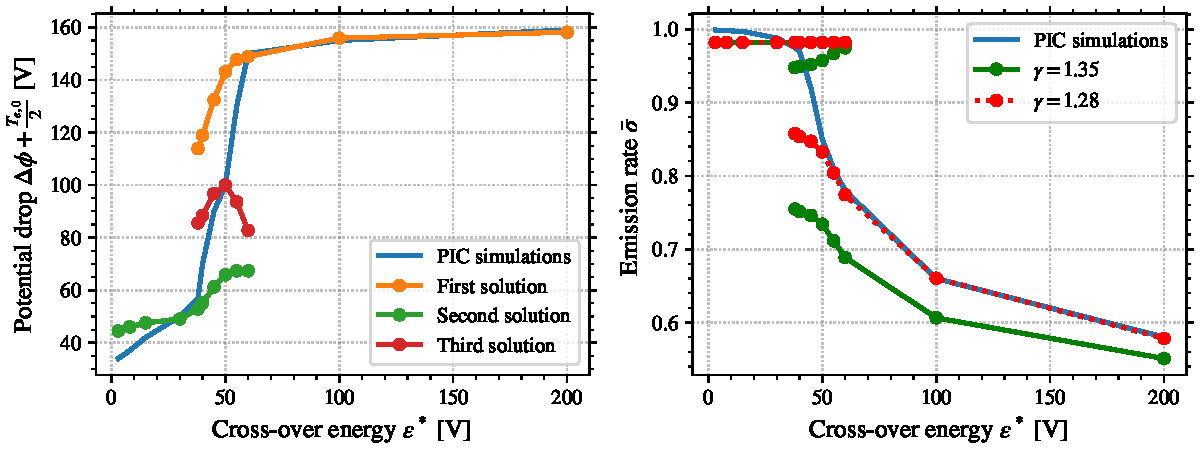
\includegraphics[width=\textwidth]{Poly_model_vs_pic}
      \caption{Comparison of the PIC simulations and the sheath model for the plasma potential drop from the center to the wall and the electron emission yield. }
      \label{fig-Poly_model_vs_pic}
    \end{figure}

    Concerning $\dphi$, we see that the sheath model combining the polytropic state law and the electron emission is in good agreement with the \ac{PIC} simulations.
    We see that the region where the three solutions coexist corresponds well with the regime {\bf II}.

    Concerning the emission rate $\rate$, we observe that the value $\gamma=1.35$ under estimates $\rate$ compared to the values of the \ac{PIC} simulations.
    On the other hand, $\gamma=1.28$ is in very good agreement.
    Interestingly, the saturation of the mean electron emission rate in the \ac{PIC} simulation is greater than the critical value $\ratecr$.
    This is because the critical value corresponds to the start of the \ac{SCL} regime, with a radial electric at the wall equals to zero.
    However, we observe in the \ac{PIC} simulation a small potential well, meaning that the \ac{SEE} rate is slightly above $\ratecr$.
    
    %\inlinenote{ As $\rate$ is better with $\gamma=1.28$, we should use both values in \cref{eq-costseepoly}. However, this increases the complexity the equations and the model, and add 1 more free parameters (they would be 2 values for $\gamma$ now). I can say that only in the discussion maybe ? }
    
  \subsection{Sheath oscillations of regime {\bf II}} \label{subsec-pic_scheath_RSO}
  
    The regime {\bf II} is characterized by the presence of oscillations between two meta-stable regimes {\bf III} and {\bf I}, one with a low emissivity and the other with a high emissivity.
    \Cref{fig-long_time} shows the temporal evolution of the electron temperature and the plasma potential relative to the wall for $\crover=45\,\volt$.
    The electron temperature is computed over the whole electron population in the \ac{PIC} simulations.
    Both the radial temperature $\Te_{,R}$ and the total temperature $\Te$ are shown (see \cref{eq-3Te} for their definition).
    The plasma potential $\dphi$ shown is measured at the center of the radial direction of the simulation, averaged over the azimuthal direction.
    
     \renewcommand\subfigurewidth{0.7\textwidth}
    \begin{figure}[!hbt]
      \centering
      \begin{tabular}{@{} c }
        \subfigure{long_time_dphi}{a}{20,20}\\
        \subfigure{long_time_Te}{b}{20,20} 
      \end{tabular}
      \caption{Temporal evolution of ({\bf a}) the plasma potential $\dphi$ and ({\bf b}) the electron temperatures\string: $\Te_{,R}$ is the radial temperature, and $\Te$ is the total temperature.}
      \label{fig-long_time}
    \end{figure}
    \renewcommand\subfigurewidth{0.47\textwidth}
    
    We clearly see in \cref{fig-long_time} the quasi-periodic oscillations between the two states.
    We observe that the electron temperature is slightly anisotropic, with the radial temperature smaller than the axial temperature.
    This anisotropy observed was not taken into account in the sheath model developed in this chapter.
    More precisely, the radial temperature $\Te_{,R}$ is linked to the thermal flux of electron toward the wall, while the total temperature $\Te$ changes the electron emission rate $\ratemaxw$.
    However, the degree of anisotropy is not very high, as it is of the order of 10\% when the sheath is not inverted.
    When the sheath is inverted, the anisotropy is of the order of 25\%, as the electron with a large radial energy are quickly absorbed.
    However in the \ac{SCL} regime, we suppose that the electron emission rate saturates at $\rate=\ratecr$, hence in this regime the impact of the total energy is less important with respect of the radial energy.
    Hence, we will compare the prediction using only the radial temperature $\Te_{,R}$ or the total, averaged, temperature $\Te$, but not the two of them together.
    
    \Cref{fig-dphi_te_PIc2} shows the potential drop as a function of the radial electron temperature $\Te_R$ and the total electron temperature $\Te = (\Te_R + \Te_{\theta} + \Te_z)/3$ measured in the \ac{PIC} simulation (same case as \cref{fig-long_time}).
    Is also shown the theoretical solutions obtained with the model of \cref{sec-fluid_poly_see} using a constant polytropic indexes $\gamma=1.35$ and $1.28$, and $\crover=45\,\volt$, and a pre-sheath potential drop of $\Teb/2$.
    
    \begin{figure}[hbt]
      \centering
      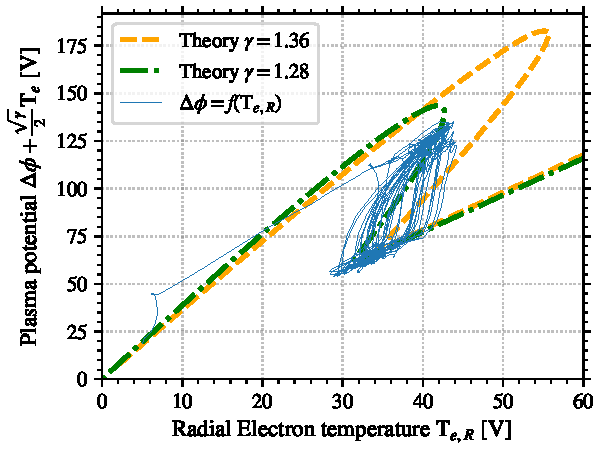
\includegraphics[width=\textwidth]{parametric_PIC_dphi_Te_two_gamma_bis}
      \caption{Plasma potential as a function of (left) the radial electron temperature $\Te_R$ and (right) the total electron temperature. The blue line is the \acs{PIC} results presented in \cref{fig-long_time}, the orange dashed lines correspond to the theoretical values with $\gamma=1.35$, and the green dotted-dashed line is computed with $\gamma=1.28$.}
      \label{fig-dphi_te_PIc2}
    \end{figure}
    % 
    % 
    % \begin{figure}[hbt]
    %   \centering
    %   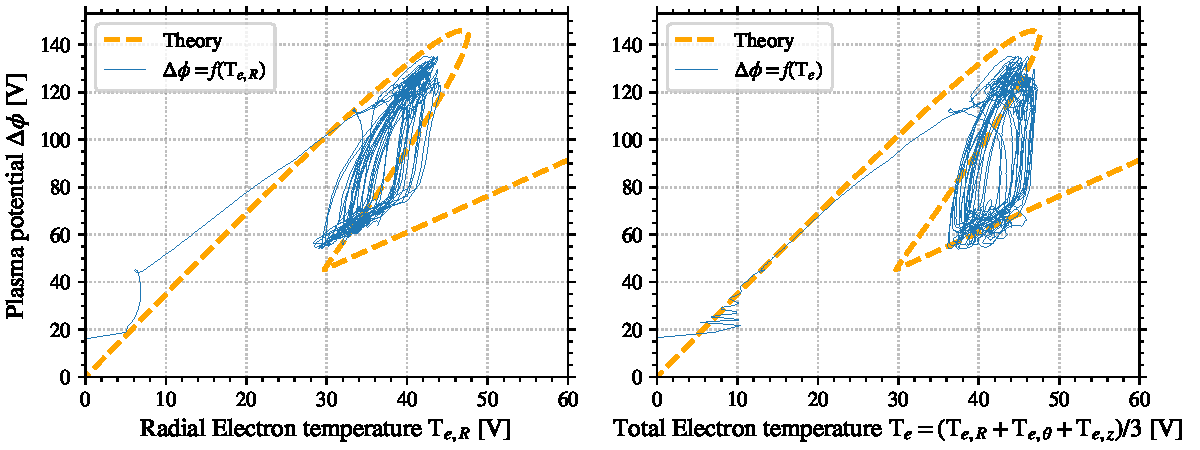
\includegraphics[width=\textwidth]{parametric_PIC_dphi_Te_bis}
    %   \caption{Plasma potential as a function of (left) the radial electron temperature and (right) the total electron temperature. The blue markers represent the \acs{PIC} results presented in \cref{fig-long_time}, and the orange dashed lines correspond to the theoretical values with $\gamma=1.35$.}
    %   \label{fig-dphi_te_PIc}
    % \end{figure}
    
    We see in \cref{fig-dphi_te_PIc2} that the sheath characteristics observed in the \ac{PIC}  simulations match relatively well the theoretically values obtained from the sheath model.
    In particular, we see the cohabitation of the two solutions of $\dphi$ observed for the same electron temperature, which corresponds to the domain of electron temperature for which the sheath model also predicts multiple solutions.
    
    During the state corresponding to regime {\bf III} (high value of  $\dphi$), the \ac{PIC} values are too noisy to clearly determine if the sheath follows the first or the second branch of the solutions.
    On the other hand, we see relatively well the correspondence between the \ac{PIC} results and the theory for the regime {\bf I} (low value of $\dphi$).
    The agreement with the polytropic sheath model using $\gamma = 1.36$ 
    
    % As discussed previously, the value of the polytropic index computed by propagating the \ac{EVDF}, is $\gamma=1.28$.
    % \Cref{fig-dphi_te_PIc2} shows the same results as \cref{fig-dphi_te_PIc}, but  the theoretical values of $\dphi$ using $\gamma=1.28$ are overlaid.
    % We see that using the value $\gamma=1.28$ does not change significantly the value of the solution, except for the maximum value of the electron temperature $\Te^1$ for the first branch of the solution, hence the domain of temperature where the three solutions coexist.
    % In the case of $\gamma=1.28$, the \ac{PIC} simulation result agreement with the theory is worse than for $\gamma=1.35$.
    
    % \begin{figure}[hbt]
    %   \centering
    %   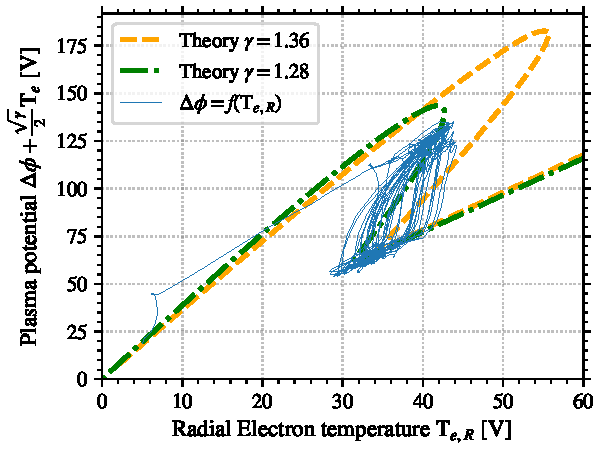
\includegraphics[width=\textwidth]{parametric_PIC_dphi_Te_two_gamma_bis}
    %   \caption{Similarly to \cref{fig-dphi_te_PIc}, Plasma potential as a function of (left) the radial electron temperature and (right) the total electron temperature. The blue markers represent the \acs{PIC} results presented in \cref{fig-long_time}, the orange dashed lines correspond to the theoretical values with $\gamma=1.35$, and the green dotted-dashed line is computed with $\gamma=1.28$.}
    %   \label{fig-dphi_te_PIc2}
    % \end{figure}
    
    \paragraph{Electron power balance\\}
    The total electron power balance integrated aver the simulation domain can be expressed as
    \begin{equation} \label{eq-GMel}
      \deriv{}{t} \lp 3/2 V n_e \Te \rp = P_{\rm abs} - P_{\rm loss},
    \end{equation}
    with $V$ the  volume of the simulation domain, $n_e$ the average electron density,  $P_{\rm abs}$ the total absorbed power, and $P_{\rm loss}$ the total power lost.
    The absorbed power $P_{\rm abs}$ is assumed to mainly be the Joule heating
    \begin{equation} \label{eq-pabs}
      P_{\rm abs} = V n_e \vect{v_e} \cdot \vect{E} = V n_e v_{e, z} E_z = V n_e \mu_e  E_z^2
    \end{equation}
    $E_z$ the imposed axial electric field and $\mu_e$ the electron axial mobility.
    From the parametric study of \cref{ch-2}, we have $\mu_e \simeq 5.6 \,\meter\squared\per\volt\per\second$.
    We observe that the absorbed power is constant.
    
    The power loss $P_{\rm loss}$ is assumed to be governed by the losses at the wall.
    Hence, as developed in \cref{sec-fluid}
    \begin{equation} \label{eq-Ploss}
      P_{\rm loss} = S \frac{1}{4} h n_e u_b 2 \Tew
    \end{equation}
    with $S$ the surface of the wall of the simulation domain, $h \sim 1$ is the ratio between the mean plasma density and the plasma density at the sheath edge, $u_b = \sqrt{\frac{\gamma e \Te}{m_i}}$ is the modified Bhom velocity and $\Tew$ is the electron temperature at the wall.
    Hence, we have
    \begin{equation} \label{eq-MG_bis}
    \frac{3}{2} \deriv{}{t} \Te = \mu_e  E_z^2 - \frac{S}{V} \frac{1}{2} \sqrt{\frac{\gamma e \Te}{m_i}}  \lp \Te - \frac{\gamma - 1}{\gamma} \dphi \rp,
    \end{equation}
    where $\frac{V}{S} = L_R$.
    \Cref{eq-MG_bis} is coupled with the sheath model that return $\dphi$ as a function of $\Te$.
    Concerning the three co-existing solutions, we assume that the sheath follows the same branch until the threshold temperature $\Te^2$, or $\Te^1$, is reached when the electron temperature increases, or decreases, respectively.
    When $\Te^1$ or $\Te^2$ is crosses, the sheath jumps to the other solution.
    
    
    \begin{figure}[!hbt]
      \centering
      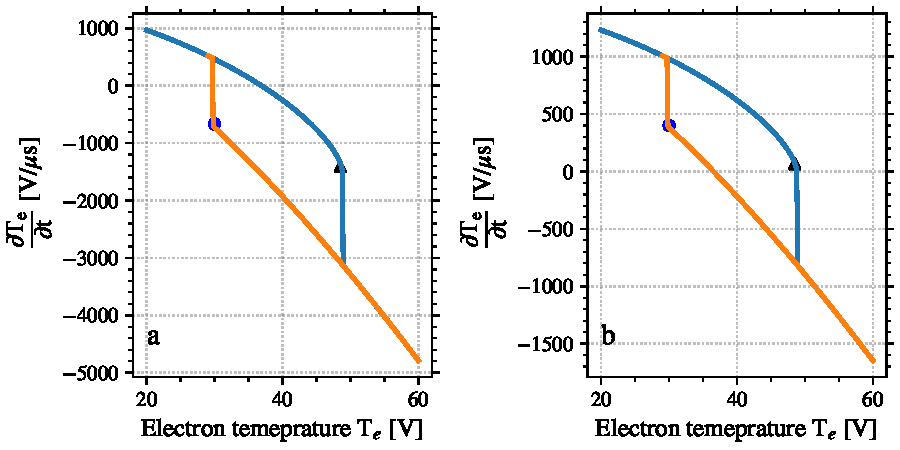
\includegraphics[width=0.9\textwidth]{Power_balance_Te.pdf}
      \caption{Evolution of the power balance $P_{\rm abs}-P_{\rm loss}$ as a function of the electron temperature for ({\bf a}) $L_R=2\,\centi\meter$ and ({\bf b}) $L_R=4\,\centi\meter$, with $\crover=45\,\volt$. The blue line corresponds to the increasing temperature for the standard sheath solution, and the orange line correspond to the decreasing temperature in the inverted sheath solution. The markers represent the limit values of the power balance.}
      \label{fig-powerbalance}
    \end{figure}
    
    \Cref{fig-powerbalance} shows the evolution of the power balance with the electron temperature for two values of $L_R=2$ and $4\,\centi\meter$.
    We see for $L_R=2\,\centi\meter$ in \cref{fig-powerbalance}.{\bf a} that starting from $\Te=20\,\volt$ the power balance is positive until $\Te\simeq36\,\volt$.
    In this condition, the system present a stable solution at that temperature.
    
    In contrast for $L_R=4\,\centi\meter$ in \cref{fig-powerbalance}.{\bf b} the power balance is positive along all of the blue curve, meaning that the electron temperature will rise until the sheath jumps to the \ac{SCL} regime.
    There, the power balance is negative, so the electron temperature will decreases until $\Te\simeq35\,\volt$ for which the power is balanced.
    
    The power balance of \cref{eq-MG_bis} cannot present an oscillating evolution, as there is a temperature for which the power is balance.
    This is because the maximum power balance in the \ac{SCL} regime (blue circle markers in  \cref{fig-powerbalance}) is above the minimum value in the standard regime (black triangular markers)
    In order to observe the oscillations, one should have the circle marker below the triangular one.
    
    % \begin{figure}[hbtp]
    %   \centering
    %   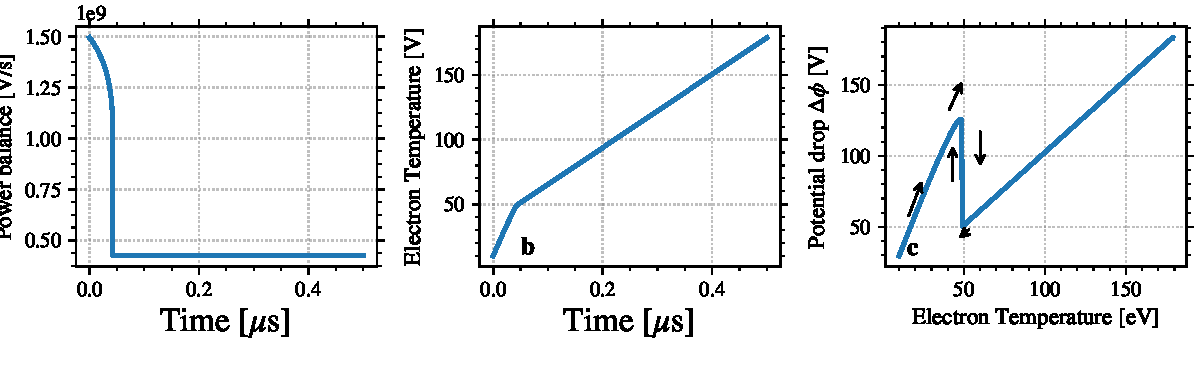
\includegraphics[width=\textwidth]{global_model.pdf}
    %   \caption{Results of the electron power balance. ({\bf a}) shows the temporal evolution of the electron power balance from \cref{eq-MG_bis}, ({\bf b}) shows the temporal evolution of the electron temperature, and ({\bf c}) shows the evolution of the plasma potential $\dphi$ as a function of $\Te$. }
    %   \label{fig-GM_results}
    % \end{figure}
    % 
    % \Cref{fig-GM_results} shows the results obtained by using the electron power balance.
    % \cref{fig-GM_results}.{\bf a} and {\bf b} shows the temporal evolution of the power balance and the electron temperature $\Te$, and \cref{fig-GM_results}.{\bf c} shows the plasma potential as a function of $\Te$.
    % Starting from an initial value $\Te=10\,\volt$, the electron temperature increases until reaching $\Te^1$.
    % Then, the sheath enters the \ac{SCL} regime and $\Te$ decreases until reaching $\Te^2$.
    % 
    % The period of the oscillation is of the order of $0.1\,\micro\second$, which is significantly shorter than the \ac{PIC} simulation.
    % Indeed, the period of the sheath oscillations observed in \cref{fig-long_time} is approximately $T = 2\,\micro\second$.
    
    \paragraph{ Ion dynamics \\}

    One has to note that the modified sheath model is stationary, while the oscillations observed are relatively fast.
    The ion dynamic can be estimated to be
    \begin{equation} \label{eq-ti}
      \tau_i = \frac{2 \pi}{\opi} = 0.1 \,\micro\second.
    \end{equation}
    
    Another estimation of the ion time scale is the time needed by an ion to reach the sheath edge from the center of the discharge.
    Supposing a constant electric field $E_{\rm ps} = \frac{\Te}{L_R}$ in the pre-sheath, we have
    \begin{equation} \label{eq-tof}
      t_{\rm flight} = L_R \sqrt{\frac{m_i}{e \Te}} = 3.7 \,\micro\second.
    \end{equation}
    with $L_R=2\,\centi\meter$ and $\Te=40\,\volt$.
    The period of the sheath oscillations observed $T = 2\,\micro\second$ is between $\tau_i$ and $t_{\rm flight}$.
    Hence, we can expect the ion dynamic to affect the plasma sheath characteristics during the sheath oscillations of the regime {\bf II}.
    
    
    The sheath oscillations of regime {\bf II} have been observed in \citet{croes2017} with three different ion masses: xenon, krypton and argon.
    The results are shown in \cref{fig-RSO_altern}.
    We see that the period of the oscillations vary with the ion mass.
    More precisely, the period of oscillation decreases with the decrease of the ion mass.
    This observation confirm that the ions have a role in the dynamics of the oscillation.
    
    \begin{figure}[hbt]
      \centering
      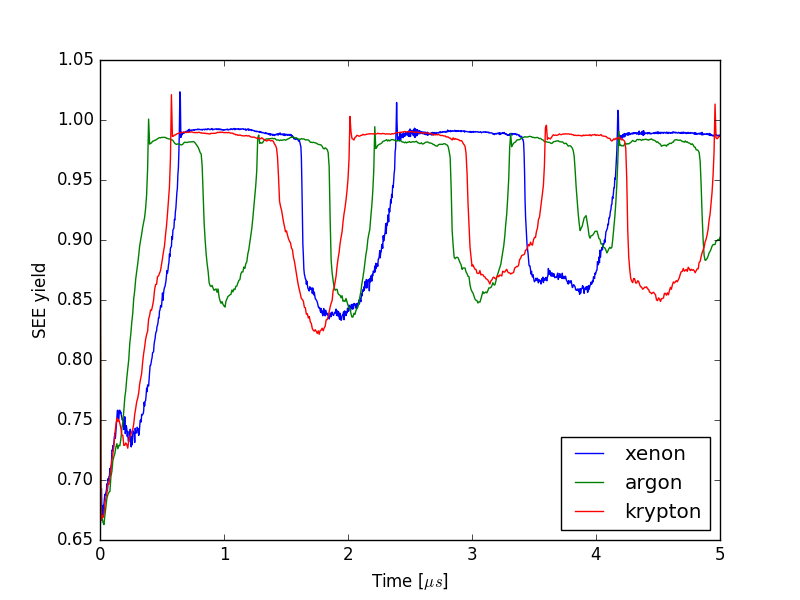
\includegraphics[width=\defaultwidth]{SEE_RSOs.png}
      \caption{Temporal evolution of the SEE rate $\rate$ measured in the PIC simulations for different gases (xenon, krypton, and argon), taken from \citet{croes2017}.}
      \label{fig-RSO_altern}
    \end{figure}
    
    